\mbox{$\displaystyle $\,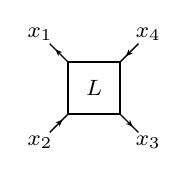
\begin{tikzpicture}[x=0.550cm, y=0.550cm, line width=0.450pt, baseline={([yshift=-0.6ex]0,0)}]
  \draw (0.000,0.000) -- (-0.600,0.600);
  \draw (0.000,0.000) -- (-0.600,-0.600);
  \draw (0.000,0.000) -- (0.600,-0.600);
  \draw (0.000,0.000) -- (0.600,0.600);
  \draw (-0.600,0.600) -- (-1.024,1.024);
  \fill (-0.889,0.889) -- (-0.825,0.730) -- (-0.814,0.814) -- (-0.730,0.825) -- cycle;
  \draw (-0.600,-0.600) -- (-1.024,-1.024);
  \fill (-0.735,-0.735) -- (-0.895,-0.799) -- (-0.810,-0.810) -- (-0.799,-0.895) -- cycle;
  \draw (0.600,-0.600) -- (1.024,-1.024);
  \fill (0.889,-0.889) -- (0.825,-0.730) -- (0.814,-0.814) -- (0.730,-0.825) -- cycle;
  \draw (0.600,0.600) -- (1.024,1.024);
  \fill (0.735,0.735) -- (0.895,0.799) -- (0.810,0.810) -- (0.799,0.895) -- cycle;
  \fill[white] (-0.600,-0.600) rectangle (0.600,0.600);
  \draw (-0.600,-0.600) rectangle (0.600,0.600);
  \node[font=\footnotesize, inner sep=0.6pt] at (0.000,0.000) {$L$};
  \node[font=\footnotesize, inner sep=0pt, anchor=315] at (-1.088,1.088) {$x_{1}$};
  \node[font=\footnotesize, inner sep=0pt, anchor=45] at (-1.088,-1.088) {$x_{2}$};
  \node[font=\footnotesize, inner sep=0pt, anchor=135] at (1.088,-1.088) {$x_{3}$};
  \node[font=\footnotesize, inner sep=0pt, anchor=225] at (1.088,1.088) {$x_{4}$};
\end{tikzpicture}}
